% Originally: content/week-02.tex, \subsection{Sequential and topological compactness agree}

\subsection{Sequential and topological compactness agree}

% Diego Torres Tejeda's supplementary note "Addendum - Sequential and Topological Compactness.pdf"
% is the one typeset document among his materials, the rest being handwritten scans. Its proof is
% adapted below into this project's notation and house style.
\begin{ainote}
Neither this equivalence nor \cref{thm:sequential_compactness} above is proved in the
transcribed notes. A complete, self-contained proof is supplied here
from a second tutor's addendum. By the reduction already noted above, compactness of
$K \subseteq X$ being compactness of the metric space $(K,d|_{K\times K})$, it suffices to treat a
whole metric space $X$ rather than a subset $K$.
\end{ainote}

\begin{lemma}[Continuous functions attain extrema on sequentially compact spaces]
\label{lem:sequential_compactness_extreme_values}
Let $(X,d)$ be sequentially compact (\cref{item:seq_compact_def963}) and $f : X \to \mathbb{R}$
continuous. Then $f$ attains a maximum and a minimum on $X$.
\end{lemma}

\begin{proof}
It suffices to find a minimum (apply the result to $-f$ for the maximum). Let
$m := \inf_{x\in X} f(x) \in [-\infty,\infty)$ and choose a sequence $(x_n)_{n}$ with
$f(x_n) \to m$. By sequential compactness, some subsequence $x_{n_k} \to x \in X$; by continuity,
$f(x) = \lim_k f(x_{n_k}) = m$. In particular $m \neq -\infty$, so $f$ attains its minimum $m$ at
$x$.
\end{proof}

\begin{remark}
This is exactly the extreme value theorem (\cref{item:extreme_value_theorem}) proved from first
principles, without presupposing \cref{thm:sequential_compactness}. Avoiding that appeal is
essential here, since that theorem is precisely what we are about to prove.
\end{remark}

\begin{definition}[Totally bounded]
\label{def:totally_bounded}
A metric space $(X,d)$ is \newterm{totally bounded} \germanfor{total beschr\"ankt} if for
every $\varepsilon > 0$ there exist finitely many points $x_1,\dots,x_n \in X$ such that
\[X = \bigcup_{k=1}^{n} B_\varepsilon(x_k).\]
\end{definition}

% Supplement: Analysis_II_Script_v1.pdf, p. 22
\begin{exercise}[Totally bounded is strictly stronger than bounded]
\label{ex:totally_bounded_implies_bounded}
Let $X$ be a metric space. Show that if $X$ is totally bounded, then it is bounded, i.e.\
$\sup_{x,x'\in X}d(x,x') < \infty$. Find an example of a bounded metric space that is
\emph{not} totally bounded.
\end{exercise}

\begin{exercisesolution}[Proof of \cref{ex:totally_bounded_implies_bounded}]
% Generator: Claude Sonnet 5 (High)
\textbf{Totally bounded $\Rightarrow$ bounded.} Apply \cref{def:totally_bounded} with
$\varepsilon := 1$: there are $x_1,\dots,x_n$ with $X = \bigcup_{k=1}^n B_1(x_k)$. Let
$M := \max_{i,j}d(x_i,x_j)$ (finite, a maximum over finitely many pairs). For any
$x,x' \in X$, choose $i,j$ with $x \in B_1(x_i)$, $x' \in B_1(x_j)$; the triangle inequality
gives $d(x,x') \leq d(x,x_i)+d(x_i,x_j)+d(x_j,x') < 1+M+1$, so $X$ is bounded.

\textbf{Not conversely.} Let $X$ be any infinite set with the discrete metric. Then
$\sup_{x,x'}d(x,x') = 1 < \infty$, so $X$ is bounded. But $X$ is not totally bounded: for
$\varepsilon := \tfrac12$, every ball $B_{1/2}(x) = \{x\}$ (\cref{def:open_ball}), so no
\emph{finite} union of such balls can cover the infinite set $X$.
\end{exercisesolution}

\begin{remark}
This is the same asymmetry \cref{lem:sequentially_compact_totally_bounded} proves in one
direction only: sequential compactness forces \emph{both} boundedness and total boundedness, and
this exercise shows the two are genuinely different hypotheses. Total boundedness is the strictly
stronger of the two, and the gap opens up in infinite dimensions.
\end{remark}

\begin{lemma}[Sequential compactness gives (total) boundedness]
\label{lem:sequentially_compact_totally_bounded}
Let $(X,d)$ be sequentially compact. Then $X$ is bounded and totally bounded
(\cref{def:totally_bounded}).
\end{lemma}

\begin{proof}
\textbf{Bounded.} Fix $x_0 \in X$; the function $f(y) := d(x_0,y)$ is continuous, so by
\Cref{lem:sequential_compactness_extreme_values} it attains a maximum $M \geq 0$ on $X$. Then
$X = B_{M+1}(x_0)$.

\textbf{Totally bounded.} Fix $\varepsilon > 0$. Construct a sequence inductively: let
$x_1 \in X$ be arbitrary, and, having chosen $x_1,\dots,x_n$, let
$U_n := \bigcup_{k=1}^n B_\varepsilon(x_k)$. If $U_n = X$, stop, since we then have the desired
finite cover. Otherwise pick $x_{n+1} \in X\setminus U_n$, so that $d(x_{n+1},x_k) \geq \varepsilon$ for
all $k \leq n$. If this process never terminates, sequential compactness gives a convergent, hence
Cauchy, subsequence $(x_{n_k})_k$; but $d(x_{n_k},x_{n_{k+1}}) \geq \varepsilon$ for all $k$
contradicts the Cauchy property. So, the process must terminate after finitely many steps, giving
the desired finite $\varepsilon$-net.

% Sonnet 5 (Medium)
\begin{center}
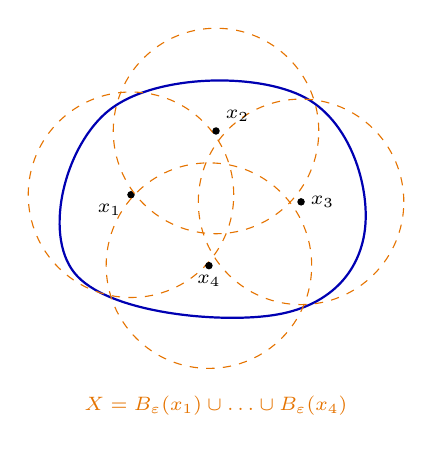
\begin{tikzpicture}[scale=0.9]
  \draw[blue!70!black, thick] plot[smooth cycle, tension=0.7] coordinates
    {(-2,-1) (-1.5,1.3) (1.2,1.5) (2.1,-0.4) (0.8,-1.6)};
  % Total boundedness means the finitely many balls really do cover X, so the
  % radius must be large enough to reach the corners of the blob.
  \foreach \p in {(-1.2,0.1),(0.0,1.0),(1.2,0.0),(-0.1,-0.9)} {
    \fill \p circle (1.5pt);
    \draw[orange!90!black, dashed] \p circle (1.45);
  }
  \node[font=\scriptsize, below left] at (-1.2,0.1) {$x_1$};
  \node[font=\scriptsize, above right] at (0.0,1.0) {$x_2$};
  \node[font=\scriptsize, right] at (1.2,0.0) {$x_3$};
  \node[font=\scriptsize, below] at (-0.1,-0.9) {$x_4$};
  \node[font=\scriptsize, orange!90!black, below] at (0,-2.6) {$X = B_\varepsilon(x_1)\cup\dots\cup B_\varepsilon(x_4)$};
\end{tikzpicture}
\end{center}
\end{proof}

\begin{theorem}[Sequential and topological compactness agree]
\label{thm:sequential_topological_compactness_equivalence}
A metric space $(X,d)$ is sequentially compact (\cref{item:seq_compact_def963}) if and only if it
is topologically compact (\cref{def:compact_metric_space}). In particular,
\Cref{thm:sequential_compactness} holds.
\end{theorem}

\begin{proof}
\textbf{($\Leftarrow$)} Suppose $X$ is not sequentially compact, so some sequence
$(x_n)_{n\in\mathbb{N}}$ has no convergent subsequence. Then no $x \in X$ is the limit of any
subsequence, so there exist $\varepsilon_x > 0$ and $N_x \in \mathbb{N}$ such that
$B_{\varepsilon_x}(x) \cap \{x_n : n \geq N_x\} = \emptyset$. The balls
$\{B_{\varepsilon_x}(x)\}_{x \in X}$ cover $X$, so topological compactness gives finitely many
$x_1,\dots,x_m$ with $X = \bigcup_{k=1}^m B_{\varepsilon_{x_k}}(x_k)$. With
$N := \max\{N_{x_1},\dots,N_{x_m}\}$, every $x_n$ with $n \geq N$ then avoids
$B_{\varepsilon_{x_1}}(x_1) \cup \dots \cup B_{\varepsilon_{x_m}}(x_m) = X$, which is absurd.
Therefore, $X$ is sequentially compact.

\begin{center}
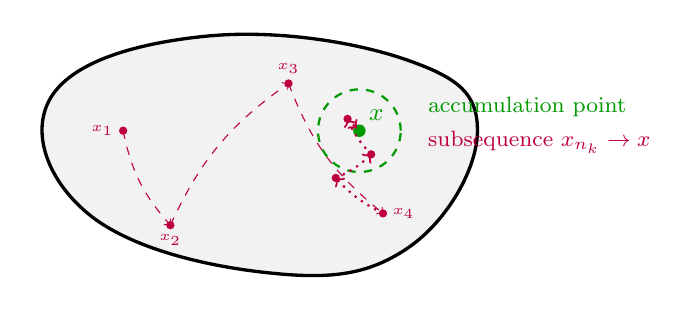
\begin{tikzpicture}[scale=1.5]
  % Space K
  \draw[very thick, fill=gray!10] plot[smooth cycle, tension=0.7] coordinates {(-1.5, -0.5) (-1.8, 0.5) (-0.5, 1) (1.2, 0.8) (1.8, 0.2) (1.2, -0.8) (0, -1)};
  
  % Sequence points and path
  \fill[purple] (-1.2, 0.2) circle (1pt) node[left] {\tiny $x_1$};
  \fill[purple] (-0.8, -0.6) circle (1pt) node[below] {\tiny $x_2$};
  \fill[purple] (0.2, 0.6) circle (1pt) node[above] {\tiny $x_3$};
  \fill[purple] (1.0, -0.5) circle (1pt) node[right] {\tiny $x_4$};
  \draw[->, purple, dashed] (-1.2, 0.2) to[bend right=15] (-0.8, -0.6);
  \draw[->, purple, dashed] (-0.8, -0.6) to[bend left=15] (0.2, 0.6);
  \draw[->, purple, dashed] (0.2, 0.6) to[bend right=15] (1.0, -0.5);
  
  % Accumulation point
  \fill[green!60!black] (0.8, 0.2) circle (1.5pt) node[above right] {\small $x$};
  \draw[green!60!black, dashed, thick] (0.8, 0.2) circle (0.35);
  
  % Subsequence converging
  \fill[purple] (0.6, -0.2) circle (1pt);
  \fill[purple] (0.9, 0) circle (1pt);
  \fill[purple] (0.7, 0.3) circle (1pt);
  \draw[->, purple, dotted, thick] (1.0, -0.5) to[bend left=10] (0.6, -0.2);
  \draw[->, purple, dotted, thick] (0.6, -0.2) to[bend right=10] (0.9, 0);
  \draw[->, purple, dotted, thick] (0.9, 0) to[bend left=10] (0.7, 0.3);
  \draw[->, purple, dotted, thick] (0.7, 0.3) -- (0.78, 0.22);
  
  \node[green!60!black, anchor=west] at (1.3, 0.4) {\footnotesize accumulation point};
  \node[purple, anchor=west] at (1.3, 0.1) {\footnotesize subsequence $x_{n_k} \to x$};
\end{tikzpicture}
\end{center}

\textbf{($\Rightarrow$)} Suppose $X$ is sequentially compact and let $\{U_i\}_{i\in I}$ be an open
cover; we may assume no single $U_i$ equals $X$ (else $\{U_i\}$ is itself a finite subcover).
Define
\[r(x) := \tfrac12\sup\{r \geq 0 : B_r(x) \subseteq U_i \text{ for some } i \in I\}, \qquad x \in X.\]
\textit{$r$ is finite and positive.} Since $\{U_i\}$ covers $X$ and each $U_i$ is open, some
$U_{i_0} \ni x$ contains a ball around $x$, so $r(x) > 0$; and since $X$ is bounded
(\cref{lem:sequentially_compact_totally_bounded}) but no $U_i$ equals $X$, $r(x) < \infty$.

\textit{$r$ is Lipschitz, hence continuous.} (That is, $|r(x)-r(y)| \leq L\,d(x,y)$ for a
constant $L$; the notion is named and placed in context as \cref{def:lipschitz_continuous},
but only the displayed estimate is used here.) Write
$R(x) := \sup\{\rho \geq 0 : B_\rho(x) \subseteq U_i \text{ for some } i\}$, so that
$r = \tfrac12 R$; it is $R$ that the argument bounds, and the factor $\tfrac12$ must be carried
through.

Let $x,y \in X$ with $d(x,y) < r(x)$. Since $r(x) < R(x)$, we have
$B_{r(x)}(x) \subseteq U_i$ for some $i$, so $y \in U_i$, and the triangle inequality gives
\[B_{r(x)-d(x,y)}(y) \subseteq B_{r(x)}(x) \subseteq U_i
\qquad\Longrightarrow\qquad R(y) \geq r(x)-d(x,y).\]
Halving, $r(y) = \tfrac12R(y) \geq \tfrac12\big(r(x)-d(x,y)\big)$, which also holds trivially
when $d(x,y) \geq r(x)$ since $r(y) \geq 0$. By symmetry,
\[|r(x)-r(y)| \leq \tfrac12\,d(x,y),\]
so $r$ is $\tfrac12$-Lipschitz, and in particular continuous, which is all that is needed below.

By \cref{lem:sequential_compactness_extreme_values}, $r$ attains a minimum
$\varepsilon := \min_{x\in X} r(x) > 0$ on $X$. Then $B_\varepsilon(x) \subseteq U_i$ for some $i$,
for every $x \in X$. By \cref{lem:sequentially_compact_totally_bounded}, $X$ is totally bounded,
so there are $x_1,\dots,x_n \in X$ with $X = \bigcup_{k=1}^n B_\varepsilon(x_k)$; choosing, for
each $k$, an index $i_k$ with $B_\varepsilon(x_k) \subseteq U_{i_k}$, the sets
$U_{i_1},\dots,U_{i_n}$ form a finite subcover of $X$.
\end{proof}

\begin{remark}[Total boundedness, more generally]
\label{rem:compact_iff_complete_totally_bounded}
Diego's note records a sharper characterization as a further exercise: $(X,d)$ is compact if and
only if it is complete and totally bounded. \Cref{lem:sequentially_compact_totally_bounded} gives
one direction (compact $\implies$ complete, by \cref{ex:compact_finite_complete} below, and
totally bounded); for the converse, a Cauchy subsequence can be extracted from any sequence using
total boundedness (cover by finitely many $\tfrac1k$-balls for $k=1,2,\dots$ and pass to nested
subsequences), and it converges by completeness.
\end{remark}

% Quelle: Diego Torres Tejeda/Addendum - Sequential and Topological Compactness.pdf, \S4(b)
\begin{definition}[Lebesgue number]
\label{def:lebesgue_number}
Let $(X,d)$ be a metric space and $\{U_i\}_{i\in I}$ an open cover of $X$. A number
$\varepsilon > 0$ is a \newterm{Lebesgue number} \germanfor{Lebesgue-Zahl} for the cover if
\[\forall x \in X\ \exists i \in I: B_\varepsilon(x) \subseteq U_i.\]
\end{definition}

\begin{remark}[Lebesgue's covering lemma]
The proof of \cref{thm:sequential_topological_compactness_equivalence} ($\Rightarrow$) shows
more than stated: on a compact metric space, \emph{every} open cover has a Lebesgue number (take
$\varepsilon := \min_{x\in X} r(x)$ as constructed there). This is known as \newterm{Lebesgue's
covering lemma} \germanfor{Lebesguesches \"Uberdeckungslemma}.
\end{remark}

\begin{proposition}[Compactness implies uniform continuity]
\label{prop:compact_implies_uniformly_continuous}
Let $(X,d_X)$, $(Y,d_Y)$ be metric spaces with $X$ compact, and let $f : X \to Y$ be continuous.
Then $f$ is uniformly continuous (\cref{def:uniformly_continuous}).
\end{proposition}

\begin{proof}
% Generator: Claude Sonnet 5 (Medium), after Diego Torres Tejeda/Addendum, §4(b)
Let $\varepsilon > 0$. The sets $f^{-1}(B_{\varepsilon/2}(y))$, $y \in Y$, are open
(\cref{def:continuous}) and cover $X$, so they admit a Lebesgue number $\delta > 0$
(\cref{def:lebesgue_number}). For any $x,x' \in X$ with $d_X(x,x') < \delta$, the ball
$B_\delta(x)$ lies inside some $f^{-1}(B_{\varepsilon/2}(y))$, so $x' \in B_\delta(x)$ gives
$f(x),f(x') \in B_{\varepsilon/2}(y)$, hence $d_Y(f(x),f(x')) < \varepsilon$ by the triangle
inequality. Since $\delta$ did not depend on $x$, $f$ is uniformly continuous.
\end{proof}

% Supplement: Sascha Brack/Class Notes/Week_02_Notes_Friday_Updated.pdf, p. 6
\begin{proposition}[A closed subset of a compact set is compact]
\label{prop:closed_subset_of_compact}
Let $(X,d)$ be a metric space, $K \subseteq X$ compact, and $A \subseteq K$ closed in $X$. Then
$A$ is compact.
\end{proposition}

\begin{proof}
Let $\mathcal{U}$ be an open cover of $A$. Since $A$ is closed, $X\setminus A$ is open, so
\[\mathcal{U}' := \mathcal{U} \cup \{X\setminus A\}\]
is an open cover of $K$, covering $A$ by assumption and everything outside $A$ by the added
set. Compactness of $K$ gives a finite subcover
$U_{1},\dots,U_{m} \in \mathcal{U}'$ of $K$, hence of $A$.

\begin{center}
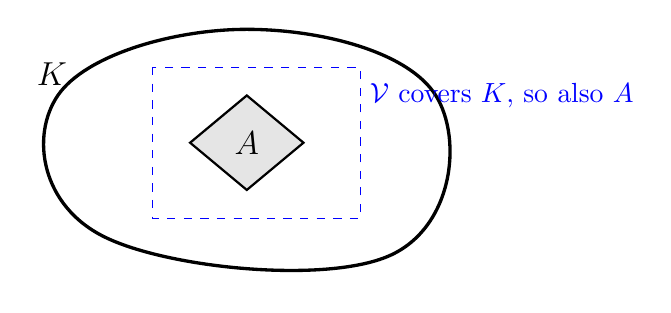
\begin{tikzpicture}[scale=1.2]
  % Compact set K
  \draw[very thick] plot[smooth cycle, tension=0.7] coordinates {(-1.5, -1) (-2, 0.5) (0, 1.2) (2, 0.5) (1.5, -1.2)};
  \node[above left, font=\large] at (-1.8, 0.5) {$K$};
  
  % Closed set A
  \draw[thick, fill=gray!20] (0, 0.5) -- (-0.6, 0) -- (0, -0.5) -- (0.6, 0) -- cycle;
  \node[font=\large] at (0, 0) {$A$};
  
  % Open cover V
  \draw[dashed, blue] (-1, 0.8) rectangle (1.2, -0.8);
  \node[blue, right] at (1.2, 0.5) {$\mathcal{V}$ covers $K$, so also $A$};
\end{tikzpicture}
\end{center}

Now simply discard $X\setminus A$ from that list if it occurs: it contains no point of $A$, so
the remaining sets still cover $A$. They all belong to $\mathcal{U}$, and there are finitely
many. As $\mathcal{U}$ was arbitrary, $A$ is compact.
\end{proof}

% Reclassified from ainote to remark: a proof technique worth naming is mathematics.
\begin{remark}[Enlarge the cover, then discard the extra set]
The trick just used is the standard way to transfer compactness downward, and it is worth
remembering in the form \emph{enlarge the cover by the complement of the set you care about, then
throw that complement away again}. It reappears whenever one needs a compact subset of a compact
set. Note that the hypothesis \qt{closed} is essential, since $(0,1) \subseteq [0,1]$ sits inside
a compact set without being compact.
\end{remark}

% Source: Corsin Nick/Class Notes/Week 2.pdf, p. 15
\begin{exercise}[Compact sets are complete]
\label{ex:compact_finite_complete}
Let $(X,d)$ be a metric space.
\begin{enumerate}[label=\textbf{(\alph*)}]
  \item Show that every finite subset $\{x_1, \dots, x_n\} \subseteq X$ is compact.
  \item If $X$ is compact, is it complete (\cref{def:complete_metric_space})?
\end{enumerate}
\end{exercise}

% Kept inline: solved directly in Corsin Nick/Class Notes/Week 2.pdf, p. 15. (The chapter-level
% "pp. 1--13" Source comment above predates this exercise; the PDF actually runs to p. 16+.)
\begin{exercisesolution}[Proof of \cref{ex:compact_finite_complete}]
\begin{enumerate}[label=\textbf{(\alph*)}]
  \item Let $\{U_\alpha\}_{\alpha \in I}$ be an open cover of $\{x_1, \dots, x_n\}$. For each
    $i = 1, \dots, n$, pick $U_{\alpha_i}$ such that $x_i \in U_{\alpha_i}$. Then
    $\{U_{\alpha_i}\}_{i=1,\dots,n}$ is a finite subcover.
  \item \textbf{Yes.} Let $(x_n)_{n=0}^{\infty}$ be a Cauchy sequence in $X$. Then, because $X$ is
    compact, we can extract a convergent subsequence such that $\lim_{i \to \infty} x_{n_i} = x \in X$.

    Fix $\varepsilon > 0$. We find $N_1 \in \mathbb{N}$ such that
    \[d(x_n, x_m) < \varepsilon \quad \forall n, m > N_1\]
    and $N_2 \in \mathbb{N}$ such that
    \[d(x, x_{n_i}) < \varepsilon \quad \forall i > N_2.\]
    Let $N := \max\{N_1, N_2\}$. For any $k > N$, we have:
    \[d(x, x_k) \leq d(x, x_{n_k}) + d(x_{n_k}, x_k) < 2\varepsilon\]
    where we used the fact that $n_k \geq k > N$. Thus, any Cauchy sequence converges.
\end{enumerate}
\end{exercisesolution}

% Moved here from after the two aiexercises below (review item D3): its "above" pointed
% past them to this solution, which is what it actually comments on.
\begin{ainote}
Corsin writes $n_k > k$ above; for a subsequence the standing fact is $n_k \geq k$. Immaterial to
the argument.
\end{ainote}

% Source: Jérôme Paschoud/Notizen/Woche 3.1 Banach und Kompaktheit.pdf, p. 3
% Generator: Gemini 3.6 Flash (High)
\begin{exercise}[Compactness of a convergent sequence]
\label{ex:convergent_sequence_compact}
Let $(X,d)$ be a metric space. Let $(x_n)_{n=0}^\infty$ be a sequence such that $x_n \to \bar{x}$. Prove that the set
\[E := \{x_n \mid n \in \mathbb{N}\} \cup \{\bar{x}\}\]
is compact.
\end{exercise}

\begin{exercisesolution}[Proof of \cref{ex:convergent_sequence_compact}]
Using topological compactness: Let $\{U_i\}_{i \in I}$ be an open cover of $E$. Since $\bar{x} \in E$, there exists some $i_* \in I$ such that $\bar{x} \in U_{i_*}$. Because $U_{i_*}$ is open and $x_n \to \bar{x}$, there exists $N \in \mathbb{N}$ such that $x_n \in U_{i_*}$ for all $n \geq N$. For the remaining finitely many points $x_0, \dots, x_{N-1}$, we can pick sets $U_{i_0}, \dots, U_{i_{N-1}}$ from the cover containing each of them. Then $\{U_{i_*}, U_{i_0}, \dots, U_{i_{N-1}}\}$ is a finite subcover of $E$.

Using sequential compactness: Let $(y_k)_{k=0}^\infty$ be a sequence in $E$. If $(y_k)$ takes values in a finite subset of $E$, it has a constant (hence convergent) subsequence. Otherwise, it takes infinitely many distinct values from $E$, which means it must contain a subsequence of $(x_n)$ progressing towards $\bar{x}$. In either case, it contains a convergent subsequence with limit in $E$. Thus $E$ is sequentially compact, hence compact.
\end{exercisesolution}

% Source: Jérôme Paschoud/Notizen/Woche 3.1 Banach und Kompaktheit.pdf, pp. 3, 6
% Generator: Gemini 3.6 Flash (High)
\begin{exercise}[Compactness of a finite set grid]
\label{ex:finite_set_compact}
Let 
\[X := \big\{ (x,y) \in \mathbb{R}^2 \mid x,y \in \mathbb{Z} \wedge |x|,|y| \leq 3 \big\}.\]
Show that $X$ is compact.
\end{exercise}

\begin{exercisesolution}[Proof of \cref{ex:finite_set_compact}]
The set $X$ contains exactly $7 \times 7 = 49$ points, so it is finite. By \cref{ex:compact_finite_complete}, every finite subset of a metric space is compact. Alternatively, using sequential compactness (as hinted in the notes), any sequence in $X$ must take at least one value infinitely often (by the pigeonhole principle), thus it contains a constant, hence convergent, subsequence.
\end{exercisesolution}
